% MSc dissertation example file, February 2022
%
% Leave one of the documentclass lines uncommented to match your degree.
% You may remove the logo option if it causes problems.
% Do not change any other options.
% \documentclass[logo,msc,adi]{infthesis}     % Adv Design Inf
% \documentclass[logo,msc,ai]{infthesis}      % AI
% \documentclass[logo,msc,cogsci]{infthesis}  % Cognitive Sci
% \documentclass[logo,msc,cs]{infthesis}      % Computer Sci
% \documentclass[logo,msc,cyber]{infthesis}   % Cyber Sec
% \documentclass[logo,msc,datasci]{infthesis} % Data Sci
% \documentclass[logo,msc,di]{infthesis}      % Design Inf
\documentclass[logo,msc,dsti]{infthesis}    % Data Sci TI
% \documentclass[logo,msc,inf]{infthesis}     % Informatics
% \documentclass[logo,msc]{infthesis}           % degree unspecified, do not change except to add your degree
%%%%%%%%%%%%%%%%%%%%%%%%
% Understand any problems and seek approval before assuming it's ok to remove ugcheck.
\usepackage{msccheck}

% Include any packages you need below, but don't include any that change the page
% layout or style of the dissertation. By including the ugcheck package above,
% you should catch most accidental changes of page layout though.

\usepackage{microtype} % recommended, but you can remove if it causes problems
\usepackage{caption}
\usepackage{subcaption}
\usepackage{url}
\usepackage{hyperref}
\usepackage{graphicx}
\usepackage{xcolor}
\usepackage{gnuplottex}
\usepackage{tikz}
\usetikzlibrary{arrows}
\usetikzlibrary{calc}
\usetikzlibrary{positioning}
\usepackage{svg}
\usepackage{pdfpages}
\usepackage{listings}
\usepackage[ruled]{algorithm2e}

\hypersetup{colorlinks=true,linkcolor=blue,filecolor=blue,urlcolor=blue,citecolor=blue}


\begin{document}

\chapter{Example results}


\section{Replicating trAIns AI versus Admiral AI}

\begin{figure}[h]
\centering
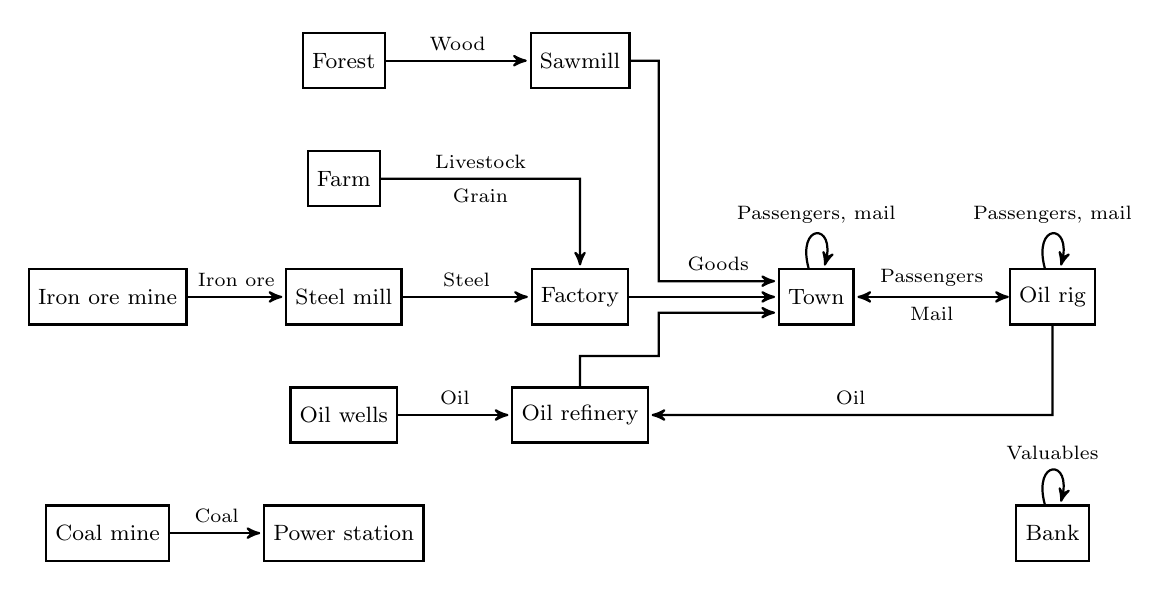
\begin{tikzpicture}[->,>=stealth',shorten >=1pt,auto,node distance=3cm,thick,main node/.style={rectangle,draw}]

    \node[main node, align=center,minimum size=0.7cm] (factory) {\footnotesize Factory};
    \node[main node, align=center,minimum size=0.7cm,on grid,right=3cm of factory] (town) {\footnotesize Town};
    \node[main node, align=center,minimum size=0.7cm,on grid,right=3cm of town] (oil-rig) {\footnotesize Oil rig};
    \node[main node, align=center,minimum size=0.7cm,on grid,left=3cm of factory] (steel-mill) {\footnotesize Steel mill};
    \node[main node, align=center,minimum size=0.7cm,on grid,left=3cm of steel-mill] (iron-ore-mine) {\footnotesize Iron ore mine};
    \node[main node, align=center,minimum size=0.7cm,on grid,below=1.5cm of steel-mill] (oil-wells) {\footnotesize Oil wells};
    \node[main node, align=center,minimum size=0.7cm,on grid,above=1.5cm of steel-mill] (farm) {\footnotesize Farm};
    \node[main node, align=center,minimum size=0.7cm,on grid,above=1.5cm of farm] (forest) {\footnotesize Forest};
    \node[main node, align=center,minimum size=0.7cm,on grid,below=3cm of oil-rig] (bank) {\footnotesize Bank};
    \node[main node, align=center,minimum size=0.7cm,on grid,below=1.5cm of oil-wells] (power-station) {\footnotesize Power station};
    \node[main node, align=center,minimum size=0.7cm,on grid,left=3cm of power-station] (coal-mine) {\footnotesize Coal mine};
    \node[main node, align=center,minimum size=0.7cm,on grid,right=3cm of forest] (sawmill) {\footnotesize Sawmill};
    \node[main node, align=center,minimum size=0.7cm,on grid,below=1.5cm of factory] (oil-refinery) {\footnotesize Oil refinery};

    \path[every node/.style={font=\scriptsize}]
        (forest) edge[] node[] {Wood} (sawmill)
        (bank) edge [loop above, distance=0.6cm] node[] {Valuables} (bank)
        (coal-mine) edge[] node[] {Coal} (power-station)
        (iron-ore-mine) edge[] node[] {Iron ore} (steel-mill)
        (oil-wells) edge[] node[] {Oil} (oil-refinery)
        (oil-rig) edge[loop above, distance=0.6cm] node[] {Passengers, mail} (oil-rig)
        (factory) edge[] node[] {} (town)
        (steel-mill) edge[] node[] {Steel} (factory)
        (town) edge[loop above, distance=0.6cm] node[] {Passengers, mail} (town);

    \path[draw,->] 
    (oil-rig.south)
    -- ($ (oil-rig.center) - (0,1.5) $)
    -- node[above] {\scriptsize Oil}
    (oil-refinery.east);

    \path[draw,<->] 
    (oil-rig.west)
    -- node[above] {\scriptsize Passengers} node[below] {\scriptsize Mail} 
    (town.east);

    \path[draw,->] 
    (farm.east)
    -- node[above] {\scriptsize Livestock} node[below] {\scriptsize Grain} ($ (farm.center) + (3,0) $)
    --
    (factory.north);

   \path[draw,->] 
    (oil-refinery.north)
    -- ($ (oil-refinery.center) + (0,0.75) $)
    -- ++(1,0)
    -- ++(0,0.55)
    -- ($ (town.west) - (0,0.2) $);

    \path[draw,->] 
    (sawmill.east)
    -- ($ (sawmill.center) + (1,0) $)
    -- ++(0,-2.8)
    -- node[above] {\scriptsize Goods} ($ (town.west) + (0,0.2) $);

\end{tikzpicture}
\caption{The possible supply chains of the temperate climate of OpenTTD 13.4, showing what types of cargo industries and towns accept and produce. Adapted from \cite{TemperateFlowChart}.}
\label{figure:temperate-supply-chains}
\end{figure}


\end{document}
